\section{Sewer reservoir}\label{se:sewer_reservoir}
In this section the model for a reservior will be explained. 

In figure \ref{fig:tank_model} an illustration of a reservoir is shown.
\begin{figure}[H]
\centering
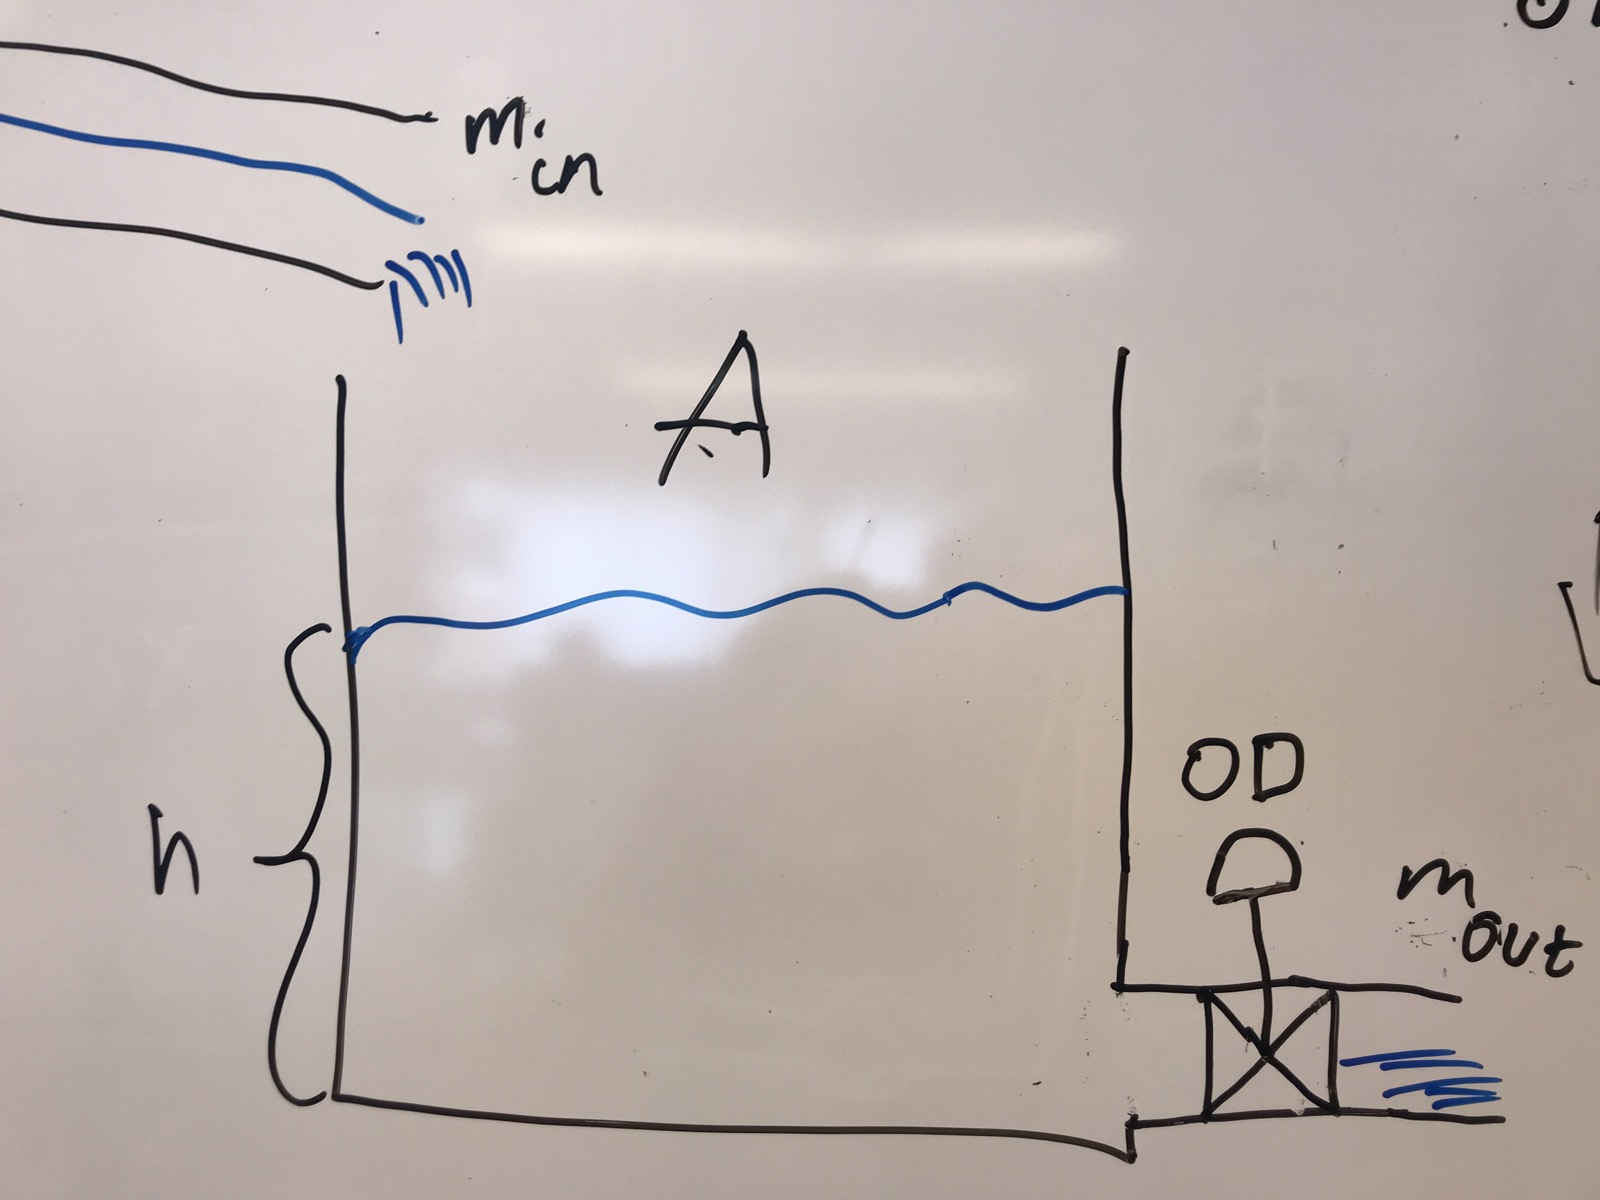
\includegraphics[width=.6\textwidth]{report/modeling/pictures/tank_model.jpg}
\caption{A illustration of a wastewater reservoir.}
\label{fig:tank_model}
\end{figure} 

This illustration will be used to derive the model for the reservior. From left we have an open channel that discharge the wastewater into the tank. The wastewater have a mass flow rate, $m_{in}$. Within the tank the wastewater has a height, h, and the reservoir has an area, A. To the bottom right the wastewater is discharged, $m_{out}$. This output mass flow is depended on the openings degree (OD) of the valve. The mass balance equation is \cite{model_tank}.

%Assumption: incompressible flow

\begin{equation}
	 	\frac{dM_{cv}(t)}{dt}=\dot{m}_{in}(t)-\dot{m}_{out}(t)
\end{equation} 

Where $M_{cv}$ is the total mass within the tank [kg], and $m_{in}$ and $m_{out}$ is the mass flow rate into the tank and away from it, $\left[\frac{kg}{s}\right]$. Total mass balance can be written as $M_{cv} = \rho Ah$ where $\rho$ is the densisty $\left[\frac{kg}{m^3}\right]$, A is the area $\left[m^2\right]$ and h is the height [m]. The mass flow rate can be written as $m = \rho Q$, where Q is the flow $\left[\frac{m^3}{s}\right]$. Thereby the following is obtained.

\begin{equation}
		\frac{d(\rho Ah(t))}{dt}=\rho Q_{in}(t)-\rho Q_{out}(t)
\end{equation}

By assuming constant density the following is obtained.

\begin{equation}\label{eq:balance_reservior}
	\rho A\frac{dh(t)}{dt}=\rho \left(Q_{in}(t)-Q_{out}(t)\right)
\end{equation}
Simplifying equation \ref{eq:balance_reservior}.

\begin{equation}\label{eq:balance_reserviorv2}
	\frac{dh(t)}{dt}=\frac{1}{A} \left(Q_{in}(t)-Q_{out}(t)\right)
\end{equation}

The output flow is, as previous mentioned, depended on the OD of the valve. Therefore a model is needed to described the output flow of the valve. The model for the valve is \cite{boysen}.
\begin{equation}\label{eq:valve_model}
	Q_{out} = kv(OD) \sqrt{\Delta p}
\end{equation}
Where kv(OD) is a function that describes the flow for different ODs. $\Delta p$ is the pressure across the valve [Pa]. The pressure at the bottom of the tank can be found with.

\begin{equation}\label{eq:pressure_at_depth}
 	P_1 = P_0 +\rho g h
 \end{equation} 
 Where $P_0$ is the atmosphere pressure $[Pa]$ and g gravitational constant $\left[\frac{m}{s^2}\right]$. The pressure on the output side of the valve is assumed to be 1 atm as it is an open channel. Inserting equation \ref{eq:pressure_at_depth} into equation \ref{eq:valve_model} the following is obtained.    


\begin{equation}\label{eq:valve_modelv2}
	Q_{out} = kv(OD) \sqrt{(P_0 +\rho g h)- P_0} = kv(OD) \sqrt{\rho g h} 
\end{equation}

Equation \ref{eq:valve_modelv2} can be inserted into equation \ref{eq:balance_reserviorv2} and thereby the following model for the reservoir is obtained.

\begin{equation}\label{eq:balance_reserviorv3}
	\frac{dh(t)}{dt}=\frac{1}{A} \left(Q_{in}(t)-\left(kv(OD) \sqrt{\rho g h(t)}\right)\right)
\end{equation}
